\chapter{Coil-array WPT}
% \chaplab{result}
% 通过上一章节的讲解,我们知道了无线传输系统在水下的基本表现。这章将介绍我们设计出的水下线圈组wpt系统,通过将大型的双线圈结构降解为多个小线圈结构,这使得内部线圈里面的磁场大幅减小,从而实现对AUV系统内部的电磁保护。
Through the explanation in the previous chapter, we know the basic performance of the wireless transmission system underwater. This chapter will introduce the underwater coil-array WPT system we designed, by degrading a large double coil structure into multiple mini-coils structures, as shown in figure \ref{fig:3_coil_array_structure}. This greatly reduces the magnetic field in the internal coil, thereby achieving electromagnetic protection inside the AUV system. Its detailed parameters are shown in table \ref{table: coil array parameters}.

\begin{figure}[!b]
    \centering
    \includegraphics[width=0.7\linewidth]{images/3_coil_array_structure.png}
    \caption{Coil-array structure.}
    \label{fig:3_coil_array_structure}
\end{figure}

% 参数表格
\begin{table}[!t]
    \centering
    \caption{The parameters of coil-array structure.}
    \begin{tabular}{ c|cc }
        \thickhline
        % \hline
        \textbf{Items}         & \textbf{Parameters}      \\
        \thickhline
        Tx coil diameter       & 160mm                    \\ \hline
        Rx coil diameter       & 100mm                    \\ \hline
        The number of Tx coils & 10                       \\ \hline
        The number of Rx coils & 5                        \\ \hline
        Mini-coil connection        & In series                \\ \hline
        Mini-coil model             & WE 760308110 (Litz wire) \\ \hline
    \end{tabular}
    \label{table: coil array parameters}
\end{table}

In the marine environment, we can use buoys to generate electricity \cite{Orekan}, store the collected electricity in the power source, and then connect the power source to the transmitter (Tx). When the AUV (Rx) reaches the designated position of the transmitter, the AUV can be charged wirelessly. This is the basic workflow of this UWPT system.
Figure \ref{fig:3_coil_array_uwpt} shows a schematic diagram of the UWPT system.

\begin{figure}[!t]
    \centering
    \includegraphics[width=0.5\linewidth]{images/3_coil_array_uwpt.png}
    \caption{Sechematic diagram of coil-array UWPT system.}
    \label{fig:3_coil_array_uwpt}
\end{figure}
In the following subsections, the performance of the coil-array UWPT system will be described in detail.


\section{Measurement of the coil-array WPT system}

In this section, we will first introduce different coil arrangements. By changing the coil structure of the coil-array, observe the performance of the changed coil structure under different conditions.

As shown in figure \ref{fig: 10-5 with ferrite}, a transmitter coil with a radius of 80mm is used here, which consists of 10 coils with ferrite in series, and a receiver coil with a radius of 50mm, which consists of 5 coils with ferrite in series. Therefore, the distance between Tx and Rx is 30mm. For other specific parameters, please find in the figure \ref{fig: 10-5 with ferrite}.

\begin{figure}[!t]
    \centering
    \includegraphics[width=1.0\linewidth]{images/4_coil_5_10_with_ferrite.png}
    \caption{Coil-array IPT structure (Both sides with ferrite tile), inner coil in the center or the outer coil.}
    \label{fig: 10-5 with ferrite}
\end{figure}
By using LCR meter to measure this arrangement system, we can get the inductance of the Tx's coil-array coil, $L_1 = 241.03 \mu H$, and quality factor $Q_1=206.25$. And the inductance of Rx's coil-array coil, $L_2 = 125.01 \mu H$, and quality factor $Q_2=207$. Then short-circuit the Rx coil and place it in the middle of the Tx coil, and measure the inductance of the Tx in this state (As shown in figure \ref{fig: Ls}), which is $L_s$, where $L_s = 240.65 \mu H$.

\begin{figure}[!b]
    \centering
    % 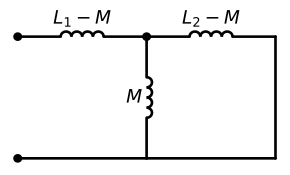
\includegraphics{images/3_mutual_inductance.png}
    \begin{tikzpicture}[scale=1, every node/.style={scale=1}, american voltages]
        \draw
        (1.5,3.5)
        to [short, o-] (4,3.5)
        to [L, l=$L_1$] (4,0)
        to [short, -o] (1.5,0);
        %\draw(-0.5,3.5) to [L,l=$M$] (-0.5,0);

        \draw
        (6,3.5) to [L, l_=$L_2$, mirror] (6,0)
        to [short, -o] (8.5,0)   ;
        \draw (8.5,3.5) to [short, o-]  (6,3.5);

        % source
        \node[below] at (5,3.5) {$M$};
        \draw [{<->}](4.234,2.6428) arc (139.9978:40:1);
    \end{tikzpicture}
    \caption{Measurement of $L_s$.}
    \label{fig: Ls}
\end{figure}

\begin{figure}[!t]
    \centering
    % 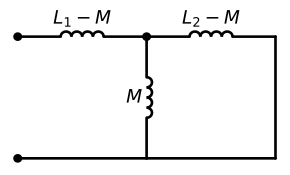
\includegraphics{images/3_mutual_inductance.png}
    \begin{tikzpicture}[scale=1, every node/.style={scale=1}, american voltages]
        \draw
        (0.75,2.75)
        to [L,l=$L_1-M$, *-] (4.5,2.75)
        to [L, l=$M$] (4.5,-1)
        to [short, -*] (0.75,-1);
        \draw
        (8.25,2.75) to [short] (8.25,-1)
        to [short] (4.5,-1)   ;
        \draw (4.5,2.75) to [L,l=$L_2-M$]  (8.25,2.75);
    \end{tikzpicture}
    \caption{Equivalent circuit of two coil model.}
    \label{fig: Ls eq}
\end{figure}

From equivalent circuit (Figure \ref{fig: Ls eq}), we can get the following formula.
\begin{equation}
    L_s = L_1 - M + \frac{M(L_2 - M)}{L_2}.
\end{equation}

Move $M$ to the left side of the equation, the mutual inductance can be expressed as,
\begin{equation}
    M = \sqrt{L_2(L_1-L_s)},
\end{equation}
and coupling coefficient,
\begin{equation}
    k = \frac{M}{L_1L_2}.
\end{equation}
$kQ$ pruduct can be expressed as,
\begin{equation}
    kQ = k\sqrt{Q_1Q_2}.
\end{equation}
$kQ$ product is an index showing the performance of a wireless transfer. The relationship between the maximum transmission efficiency $\eta_{max}$ and $kQ$ as follows \cite{Li2015, Ohira2014},
\begin{equation}
    \eta_{max} = \frac{k^2Q_1Q_2}{(1+\sqrt{1+k^2Q_1Q_2})^2}.
\end{equation}
According to the calculation of the above formula, we can get that the maximum transmission efficiency $\eta_{max}$ of this arrangement is $78.41\%$.

\section{The other coil arrangements and comparison}
% 接下来,我们通过增加线圈个数,改变Rx线圈在Tx线圈中的位置,来观察不同条件下系统的表现。结果如下图()所示。
Next, we will observe the performance of the system under different conditions by increasing the number of coils and changing the position of the Rx coil in the Tx coil. The result is shown in the figure \ref{fig: coil-array result1}, figure \ref{fig: coil-array result2}, and figure \ref{fig: coil-array result3}.
\begin{figure}[!b]
    \centering
    \includegraphics[width=0.65\textwidth]{images/4_coil_5_10_without_ferrite.png}
    \caption{Coil-array IPT structure (both sides without ferrite tile), inner coil in the center of the outer coil (left), inner coil next to the outer coil (right).}
    \label{fig: coil-array result1}
\end{figure}
\begin{figure}[!t]
    \centering
    \includegraphics[width=0.65\textwidth]{images/4_coil_6_10_without_ferrite.png}
    \caption{Coil-array IPT structure (both sides without ferrite tile), inner coil in the center of the outer coil (left), inner coil next to the outer coil (right).}
    \label{fig: coil-array result2}
\end{figure}
\begin{figure}[!t]
    \centering
    \includegraphics[width=0.65\textwidth]{images/4_coil_6_10_inner_with_ferrite.png}
    \caption{Coil-array IPT structure (inner small coils with ferrite tile, outer small coils without ferrite tile), inner coil in the center of the outer coil (left), inner coil next to the outer coil (right).}
    \label{fig: coil-array result3}
\end{figure}


\begin{table}[!t]
    \centering
    \caption{Maximum power transfer efficiency of different coil arrangements.}
    \resizebox*{\textwidth}{!}{
        \begin{tabular}{|>{\centering\arraybackslash}m{3.3cm}|>{\centering\arraybackslash}m{2.5cm}|>{\centering\arraybackslash}m{2.5cm}|>{\centering\arraybackslash}m{2.5cm}|>{\centering\arraybackslash}m{2.5cm}|}
            \hline
            \textbf{Shift}                                        & \textbf{Numbers of coil (Outer - Inner)} & \textbf{Both coils with ferrite} & \textbf{Both coils without ferrite} & \textbf{Outer coils without ferrite, inner coils with ferrite} \\ \hline
            \multirow{2}{3.3cm}{Inner coil in the center}         & 10 - 5                                   & 78.41\%                          & 76.75\%                             & 84.95\%                                                        \\ \cline{2-5}
                                                                  & 10 - 6                                   &                                  & 77.03\%                             &                                                                \\ \hline
            \multirow{2}{3.3cm}{Inner coil close to the one side} & 10 - 5                                   &                                  & 88.26\%                             & 78.80\%                                                        \\ \cline{2-5}
                                                                  & 10 - 6                                   &                                  & 91.13\%                             &                                                                \\ \hline
        \end{tabular}}
    \label{table: comparison of the different coil arrangement}
\end{table}

% 通过上面各个方案下的结果,我们可以将其汇总成表1,如下
Through the results under each of the above scenarios, we can summarize them into table \ref{table: comparison of the different coil arrangement}, as follows

From table \ref{table: comparison of the different coil arrangement}, we can get the following conclusions:
\begin{itemize}
    \item When we increase the number of inner coils from 5 to 6, the maximum PTE (Power transfer efficiency) will increase.
    \item If the numbers of outer and inner coils are the same, when outer coils without ferrite and inner coils with ferrite, we can get the maximum PTE.
    \item When there is no ferrite outside the inner coil, the PTE will increase if the inner coil deviates from the middle, and vice versa.
\end{itemize}

\section{Megnetic field distribution}
% 为了弄清coil-array结构的磁场分布,我们使用了Wipl-d电磁模拟软件。我们对以下两个结构进行了模拟,具体参数如下表。
In order to clarify the magnetic field distribution of the coil-array structure, we used Wipl-d electromagnetic simulation software. We simulated the following two structures as shown in figure \ref{fig: two strcture}, and the specific parameters are as table \ref{table: simulation parameters}.

\begin{table}[!t]
    \centering
    \caption{The parameters of two coil structure in simulation.}
    \begin{tabular}{ c|c|c }
        \thickhline
        % \hline
        \textbf{Items}         & \textbf{Coil-array structure} & \textbf{Two-ring structure} \\
        \thickhline
        Tx coil diameter       & 160mm                         & 160mm                       \\ \hline
        Rx coil diameter       & 100mm                         & 100mm                       \\ \hline
        The number of Tx coils & 12                            & 1                           \\ \hline
        The number of Rx coils & 8                             & 1                           \\ \hline
        Wire material          & Copper                        & Copper                      \\ \hline
        Frequency              & 200kHz                        & 200kHz                      \\ \hline
        Resistance of load     & $5 \si{\ohm}$                 & $5 \si{\ohm}$               \\ \hline
        Voltage of source      & 6v                            & 64v                         \\ \hline
        Output power           & 10w                           & 10w                         \\ \hline
    \end{tabular}
    \label{table: simulation parameters}
\end{table}

\begin{figure}[!t]
    \resizebox*{\textwidth}{!}{
        \begin{subfigure}{0.5\textwidth}
            \centering
            \includegraphics[height=6.4cm]{images/4_coil_array_system.png}
            \caption{Coil-array IPT structure.}
            \label{fig:subim1}
        \end{subfigure}
        \begin{subfigure}{0.5\textwidth}
            \centering
            \includegraphics[height=6.4cm]{images/4_two_ring_system.png}
            \caption{Two-ring IPT structure.}
            \label{fig:subim2}
        \end{subfigure}
    }
    \caption{Two kind of UWPT coil structure simulation diagram.}
    \label{fig: two strcture}
\end{figure}

\subsection{Megnetic field distribution of two-ring strcture}

\begin{figure}[!b]
    \centering
    \includegraphics[width=0.9\linewidth]{images/4_two_ring_near_field_distribution.JPG}
    \caption{Magnetic field distribution of two-ring IPT structure.}
    \label{fig: magnetic distribution of two ring}
\end{figure}

\begin{figure}[!t]
    \centering
    \includegraphics[width=0.9\linewidth]{images/4_two_ring_near_field_distribution_cut.JPG}
    \caption{Cross-sectional view of the magnetic field distribution of two-ring IPT structure.}
    \label{fig: magnetic distribution of two ring cut}
\end{figure}

% 为了判断coil-array结构是否能够减小AUV系统内部磁场强度,我们首先对传统的two-ring系统进行了模拟。
% 其结果如图1和图2所示,图一显示了在三维空间中收发线圈之间的磁场分布。其中图示最高的顶峰为两线圈的正中间,即在AUV内部会产生如图1所示的磁场分布。图二为图一从侧面划开的剖面图,我们可以看到中间部分的磁感应强度到达了83.95A/m,其他部分逐步降低,如山峰状。

In order to judge whether the coil-array structure can reduce the internal magnetic field strength of the AUV system, we first simulated the conventional two-ring structure.
The results are shown in figure \ref{fig: magnetic distribution of two ring} and figure \ref{fig: magnetic distribution of two ring cut}. figure \ref{fig: magnetic distribution of two ring} shows the magnetic field distribution between the transmitting and receiving coils in a three-dimensional space. The highest peak in the figure is the middle of the two coils, that is, the magnetic field distribution shown in figure \ref{fig: magnetic distribution of two ring} is generated inside the AUV. figure \ref{fig: magnetic distribution of two ring cut} is a cross-sectional view of figure \ref{fig: magnetic distribution of two ring} from the side. We can see that the magnetic induction intensity of the middle part has reached $83.95A/m$, and the other parts are gradually decreasing, like a mountain.

\subsection{Megnetic field distribution of coil-array strcture}

\begin{figure}[!b]
    \centering
    \includegraphics[width=0.9\linewidth]{images/4_coil_array_near_field_distribution.JPG}
    \caption{Magnetic field distribution of coil-array IPT structure.}
    \label{fig: magnetic distribution of coil array}
\end{figure}

\begin{figure}[!t]
    \centering
    \includegraphics[width=0.9\linewidth]{images/4_coil_array_near_field_distribution_cut.JPG}
    \caption{Cross-sectional view of the magnetic field distribution of aoil-array IPT structure.}
    \label{fig: magnetic distribution of coil array cut}
\end{figure}

% 在完成two-ring结构的磁场分布模拟后,我们对coil-array结构线圈做了同样的模拟,结果如图1和图2所示。
% 图一中我们可以看到coil-array结构的磁场分布像一个火山,其中间部分磁感应强度低,周围磁感应强度高。磁感应强度最高的部分为两线圈之间,即在AUV外部,不会对AUV系统内部造成影响。通过图2我们可以看出AUV内部的磁场在50A/m左右,相比与two-ring结构降低了40%,并且其大磁感应强度低于70A/m,比two-ring结构的最高磁感应强度低了13A/m。
After completing the simulation of the magnetic field distribution of the two-ring structure, we did the same simulation on the coil-array structure coil, and the results are shown in figure \ref{fig: magnetic distribution of coil array} and figure \ref{fig: magnetic distribution of coil array cut}.
In figure \ref{fig: magnetic distribution of coil array}, we can see that the magnetic field distribution of the coil-array structure is like a volcano, with low magnetic induction in the middle part and high surrounding magnetic induction. The part with the highest magnetic induction is between the two coils, that is, outside the AUV, which will not affect the inside of the AUV system. From figure \ref{fig: magnetic distribution of coil array cut} we can see that the internal magnetic field of the AUV is around 50A/m, which is 40\% lower than the two-ring structure, and its large magnetic induction intensity is lower than 70A/m, which is lower than the highest magnetic induction intensity of the two-ring structure 13A/m.


\section{PET over shift in two directions}

\begin{figure}[!t]
    \centering
    % 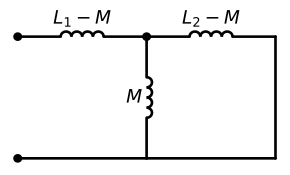
\includegraphics{images/3_mutual_inductance.png}
    \resizebox*{0.5\textwidth}{!}{
        \begin{tikzpicture}
            \draw  (-1,3) ellipse (1 and 3);
            \draw  (-1,3) ellipse (0.5 and 1.5);
            \node[single arrow,draw=black,fill=black!5,minimum height=2.5cm,shape border rotate=0] at (1.5,3) {};
            \node[single arrow,draw=black,fill=black!5,minimum height=2.5cm,shape border rotate=90] at (-3,4.5) {};
            \node[below] at (1.5,4) {Horizontal shift};
            \node[below] at (-4.5,5) {Vertical shift};
        \end{tikzpicture}
    }
    \caption{Schematic diagram of direction indication.}
    \label{fig: direction}
\end{figure}

Since both the coil-array and the two-ring are hollow cylindrical structures transmitter, the rotation of the receiver coil will not have much impact on the system transmission efficiency. This section will explore the offset effect of these two structures in the horizontal direction and vertical direction.
Suppose the horizontal offset and vertical offset are specified as shown in figure \ref{fig: direction}.

We first offset the internal coils of the two structures from 0 to 100mm in the horizontal direction to obtain the result in figure \ref{fig: PET in two directions} (a). The red line part is the coil-array structure, and the blue part is the two-ring structure. From the figure, we can find that when Rx is in the center of Tx, the transmission efficiency of the two-ring structure is 95\%, while the transmission efficiency of the coil-array structure is 60\%. And when the horizontal offset increases, the transmission efficiency of the coil-array structure changes greatly, and when the offset is 100mm, the PTE is close to 0. The PTE of the two-ring structure remains basically unchanged.

This is because the coupling of the coil-array structure is completed by small coils. When the horizontal offset exceeds the size of the coil, the opposite circular coil cannot be coupled 
well, so the PET drops sharply. The coupling of the two-ring structure is the coupling between two hollow cylindrical coils, like two solenoids, so even when a large displacement occurs in the horizontal direction, the PTE can basically remain unchanged.

Figure \ref{fig: PET in two directions} (b) shows the offset in the vertical direction. We can see that the red line representing the coil-array structure increases with the horizontal offset of the Rx coil, that is, the Tx coil and the Rx coil are getting closer, and the PTE of the system is also constantly increase. When the offset reaches 25mm, the PTE of the system is close to 90\%.

Although we found that the system transmission efficiency and anti-offset ability of the coil-array structure is not as well as the two-ring structure, but in some specific occasions (hope that the internal components of the AUV system can get good electromagnetic protection), we prefer to use the coil-array structure for power transmission.

\begin{figure}[!t]
    \centering
    \resizebox*{\textwidth}{!}{
        \begin{subfigure}[]{\textwidth}
            \resizebox*{\textwidth}{!}{
                \begin{tikzpicture}[scale=1, every node/.style={scale=1},anchor=south west]%, every node/.style={scale=1},anchor=south west]
                    \begin{axis}[xlabel={(a) Horizontal shift $[\si{\milli\meter}]$\\},ylabel={RF-RF efficiency $[\%]$},
                            legend style={
                                    at={(axis cs:97,0.7)},
                                    legend cell align={left},
                                    legend columns=1,
                                    /tikz/column 2/.style={column sep=15pt,},
                                },
                            xmin=0, xmax=100, ymin=0, ymax=1,
                            xtick = {0, 20, 40,60,80,100},
                            ytick = {0,0.20,0.40,0.60,0.80,1},
                            grid=both,
                            grid style={line width=.1pt, draw=gray!20},
                            %minor x tick num=2,
                            %minor y tick num=4,
                            ylabel near ticks,
                            line width = 0.3mm,
                            % label style={font=\large},
                            % tick label style = {font=\large},
                            legend cell align={left},]
                        \addplot[blue, mark = *, line width = 0.5mm] table[x=yshift,y=tworing] {data/PET.txt};
                        \addplot[red, mark = square*, line width = 0.5mm] table[x=yshift,y=coilarray] {data/PET.txt};
                        % \addplot[red, mark = square*, line width = 0.5mm] table {../journaldata/eff_prop_3term_15turn_d150_d260.txt};
                        %\addplot[red, mark = square*, line width = 0.5mm] table {../data/eff_prop_3term_15turn_d150_d260_relay1coil.txt};
                        %\node [align = center] at (axis cs: 40,85) {proposed (2-coil relay)}; 
                        %\node [align = center] at (axis cs: 40,55) {[1]}; % \cite{Cheng2019}
                        %\draw[-latex]  (axis cs: 72,30) node [anchor=north] {proposed (1-coil relay)} --  (axis cs: 72,67) ;
                        \legend{ two-ring structure, coil-array structure}
                    \end{axis}
                \end{tikzpicture}
            }
            % \caption{PEI over horizontal shift.}
        \end{subfigure}

        \begin{subfigure}[]{\textwidth}
            \resizebox*{\textwidth}{!}{
                \begin{tikzpicture}[scale=1, every node/.style={scale=1},anchor=south west]%, every node/.style={scale=1},anchor=south west]
                    \begin{axis}[xlabel={(b) Vertical shift $[\si{\milli\meter}]$},ylabel={RF-RF efficiency $[\%]$},
                            legend style={
                                    at={(axis cs:24.5,0.5)},
                                    legend cell align={left},
                                    legend columns=1,
                                    /tikz/column 2/.style={column sep=15pt,},
                                },
                            xmin=0, xmax=25, ymin=0, ymax=1,
                            xtick = {0, 5, 10,15,20,25},
                            ytick = {0,0.20,0.40,0.60,0.80,1},
                            grid=both,
                            grid style={line width=.1pt, draw=gray!20},
                            %minor x tick num=2,
                            %minor y tick num=4,
                            ylabel near ticks,
                            line width = 0.3mm,
                            % label style={font=\large},
                            % tick label style = {font=\large},
                            legend cell align={left},]
                        \addplot[blue, mark = *, line width = 0.5mm] table[x=xshift,y=tworing] {data/PET_xshift.txt};
                        \addplot[red, mark = square*, line width = 0.5mm] table[x=xshift,y=coilarray] {data/PET_xshift.txt};
                        % \addplot[red, mark = square*, line width = 0.5mm] table {../journaldata/eff_prop_3term_15turn_d150_d260.txt};
                        %\addplot[red, mark = square*, line width = 0.5mm] table {../data/eff_prop_3term_15turn_d150_d260_relay1coil.txt};
                        %\node [align = center] at (axis cs: 40,85) {proposed (2-coil relay)}; 
                        %\node [align = center] at (axis cs: 40,55) {[1]}; % \cite{Cheng2019}
                        %\draw[-latex]  (axis cs: 72,30) node [anchor=north] {proposed (1-coil relay)} --  (axis cs: 72,67) ;
                        \legend{ two-ring structure, coil-array structure}
                        
                    \end{axis}
                \end{tikzpicture}
            }
            % \caption{PEI over vertical shift.}
        \end{subfigure}
    }
    \caption{The PET over shift in two different directions.}
    \label{fig: PET in two directions}
\end{figure}


% \begin{figure}[!t]
%     \centering
%     \begin{tikzpicture}[scale=1, every node/.style={scale=1},anchor=south west]%, every node/.style={scale=1},anchor=south west]
%         \begin{axis}[xlabel={Resistance of load $[\si{\ohm}]$},ylabel={RF-RF efficiency $[\%]$},
%                 legend style={
%                         at={(axis cs:9.5,0.3)},
%                         legend cell align={left},
%                         legend columns=1,
%                         /tikz/column 2/.style={column sep=15pt,},
%                     },
%                 xmin=0, xmax=11, ymin=0, ymax=1,
%                 xtick = {0, 2, 4,6,8,10},
%                 ytick = {0,0.20,0.40,0.60,0.80,1},
%                 grid=both,
%                 grid style={line width=.1pt, draw=gray!20},
%                 %minor x tick num=2,
%                 %minor y tick num=4,
%                 ylabel near ticks,
%                 line width = 0.3mm,
%                 % label style={font=\large},
%                 % tick label style = {font=\large},
%                 legend cell align={left},]
%             \addplot[red, mark = square*, line width = 0.5mm] table[x=R,y=PET] {data/PET_R.txt};
%             % \addplot[red, mark = square*, line width = 0.5mm] table[x=xshift,y=coilarray] {data/PET_xshift.txt};
%             % \addplot[red, mark = square*, line width = 0.5mm] table {../journaldata/eff_prop_3term_15turn_d150_d260.txt};
%             %\addplot[red, mark = square*, line width = 0.5mm] table {../data/eff_prop_3term_15turn_d150_d260_relay1coil.txt};
%             %\node [align = center] at (axis cs: 40,85) {proposed (2-coil relay)}; 
%             %\node [align = center] at (axis cs: 40,55) {[1]}; % \cite{Cheng2019}
%             %\draw[-latex]  (axis cs: 72,30) node [anchor=north] {proposed (1-coil relay)} --  (axis cs: 72,67) ;
%             % \legend{ two-ring structure}
%         \end{axis}
%     \end{tikzpicture}
%     \caption{The PET over different resistance of load (coil-array structure).}
% \end{figure}
